\documentclass[12pt,a4paper]{article}
\usepackage[UTF8]{ctex}     %先引入ctex
\usepackage[utf8]{inputenc} %再引入inputenc
\usepackage{graphicx}
\usepackage{lazylatex}
\usepackage{amsmath}
\usepackage{bookmark}
\usepackage{enumerate}
\tcbuselibrary{documentation}
\graphicspath{{img/}}
% 边距
\geometry{left=2.0cm,right=2.0cm,top=2.0cm,bottom=3.0cm}
% 大题
\newenvironment{problems}{\begin{list}{}{\renewcommand{\makelabel}[1]{\textbf{##1}.\hfil}}}{\end{list}}
% 小题
\newenvironment{steps}{\begin{list}{}{\renewcommand{\makelabel}[1]{(##1)\hfil}}}{\end{list}}
% 答
\providecommand{\ans}{\textbf{答}:~}
% 解
\providecommand{\sol}{\textbf{解}.~}

\renewcommand{\theFancyVerbLine}{\ttfamily
\textcolor[rgb]{0.5,0.5,1.0}{\tiny
\oldstylenums{\arabic{FancyVerbLine}}}}

\begin{document}
\title{\normalsize \underline{计算机系统结构(A)}\\\LARGE 实验 1}
\author{Log Creative }
\date{\today}
\maketitle

\begin{problems}
    \item[0] \textbf{准备操作}
    解压缩操作
    \begin{code}{shell}
        tar --get -f lab0.tar.gz
    \end{code}
    \item[1] \texttt{gcc} 修改\fname{glory.c}宏参数为
    \begin{code}{c}
/* Only change any of these 4 values */
#define V0 3
#define V1 3
#define V2 1
#define V3 3
    \end{code}
    运行结果如下:

    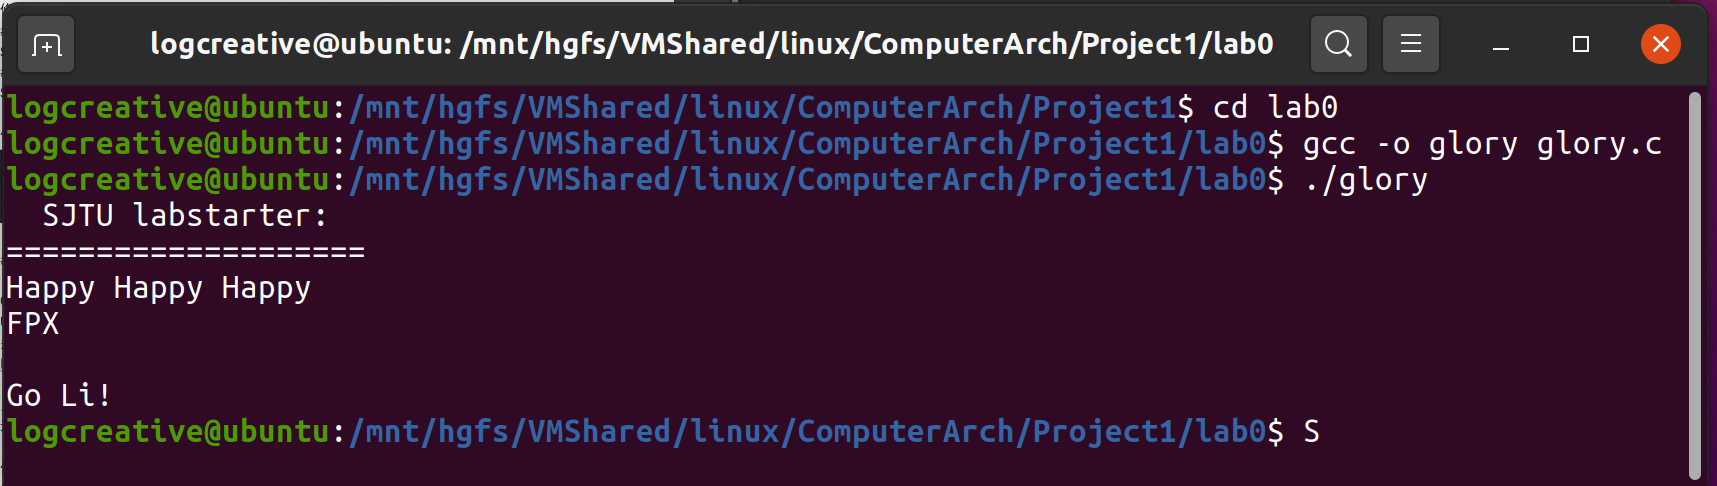
\includegraphics[width=0.9\textwidth]{gcc.png}

    \item[2] \texttt{gdb}
    \begin{enumerate}[(1)]
        \item How do you pass command line arguments to a program when using gdb?
        
        \ans 在编译时添加 \texttt{-g} 的指令,以期调试。
        \begin{code}{shell}
            gcc -g -o hello hello.c
            gdb hello
        \end{code}

        \item How do you set a breakpoint which only occurs when a set of conditions is true (e.g. when certain variables are a certain value)?
        
        \ans 进入 \texttt{gdb} 环境后,采用如下命令对变量 \texttt{ch} 进行监视,当其变为 e 的时候触发第 12 行的断点。这样就设置了条件断点。
        \begin{code}{shell}
            (gdb) break 12 if ch=='e'
        \end{code}

        \item How do you execute the next line of C code in the program after stopping at a breakpoint?
        
        \ans 使用单步调试命令:
        \begin{code}{shell}
            (gdb) next
        \end{code}
        并且持续回车可以持续单步调试。

        \item If the next line of code is a function call, you'll execute the whole function call at once if you use  your  answer  to (3).  How  do  you  tell GDB that  you  want  to  debug  the  code inside  the function instead?
        
        \ans 直接传入函数参数作为断点:
        \begin{code}{shell}
            (gdb) break main
        \end{code}

        \item How do you resume the program after stopping at a breakpoint?
        
        \ans 使用继续命令:
        \begin{code}{shell}
            (gdb) continue
        \end{code}
        并且持续回车可以连续继续。

        \item How can you see the value of a variable (or even an expression like 1+2) in gdb?
        
        \ans 在设置完断点后,运行,中断时使用 \texttt{print} 打印 \texttt{ch} 或 \texttt{ch+1} 的值:
        \begin{code}{shell}
            (gdb) break 12
            (gdb) run
            (gdb) print ch
            $1 = 108 'l'
            (gdb) print ch+1
            $2 = 109
            (gdb) continue
        \end{code}

        \item How do you configure gdb so it prints the value of a variable after every step?
        
        \ans 在设置完断点后,运行,中断时使用 \texttt{awatch} 指令监视 \texttt{ch} 或 \texttt{ch+1} 的值:
        \begin{code}{shell}
            (gdb) run
            (gdb) awatch ch
            (gdb) awatch ch+1
            (gdb) continue
        \end{code}

        就在每次中断后收到如下的信息:
        
        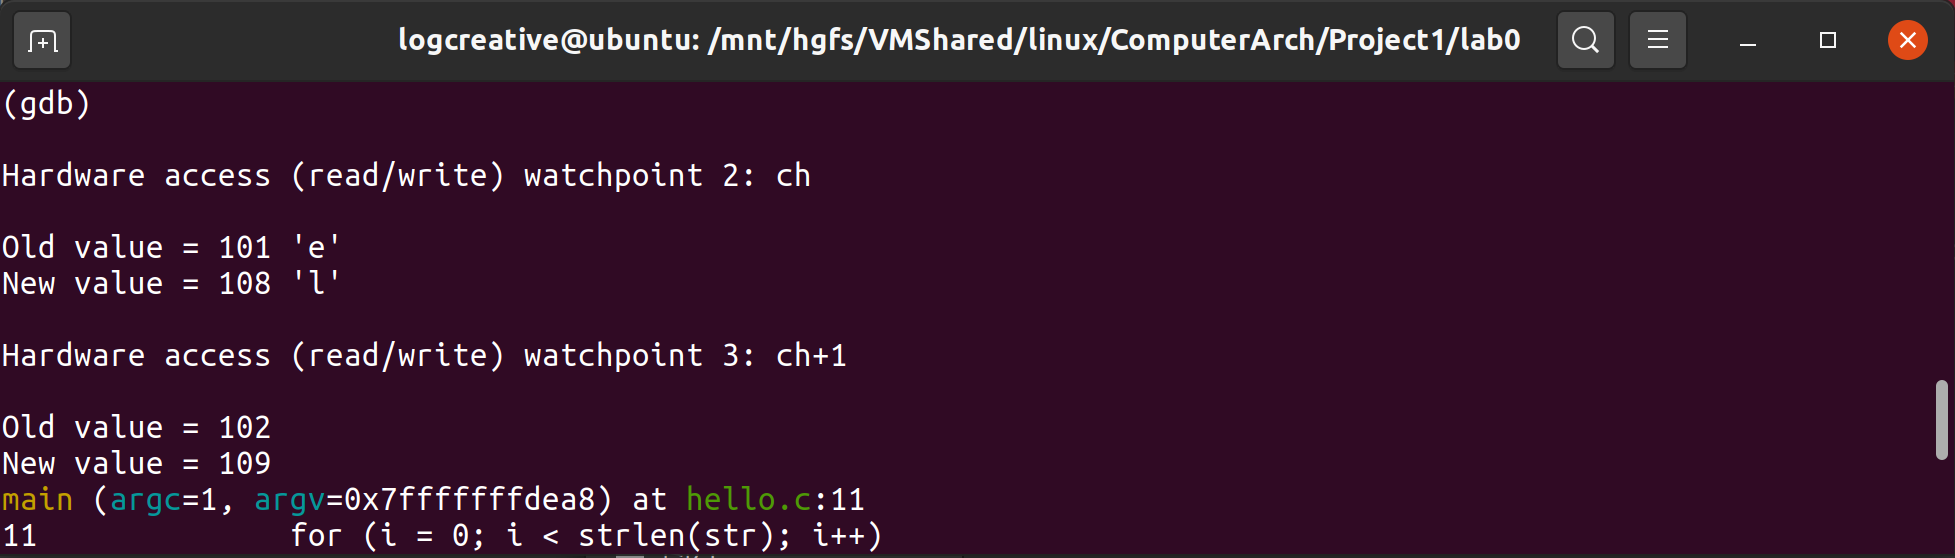
\includegraphics[width=0.8\textwidth]{awatch.png}

        \item How do you print a list of all variables and their values in the current function?
        
        \ans 在运行中断后,使用下述命令打印所有的局部变量:
        \begin{code}{shell}
            (gdb) info locals
            i = 0
            str = 0x555555556004 "hello, world!"
            ch = 0 '\000'
        \end{code}

        \item How do you exit out of gdb?
        
        \ans 使用退出指令:
        \begin{code}{shell}
            (gdb) quit
        \end{code}
    \end{enumerate}
    

    \item[3] \textbf{调试}
    
    \ans 编译完成后进入 \texttt{gdb} 调试,在第 10 行处打下断点,并监视变量 \texttt{a} 和 \texttt{b} 的值。

    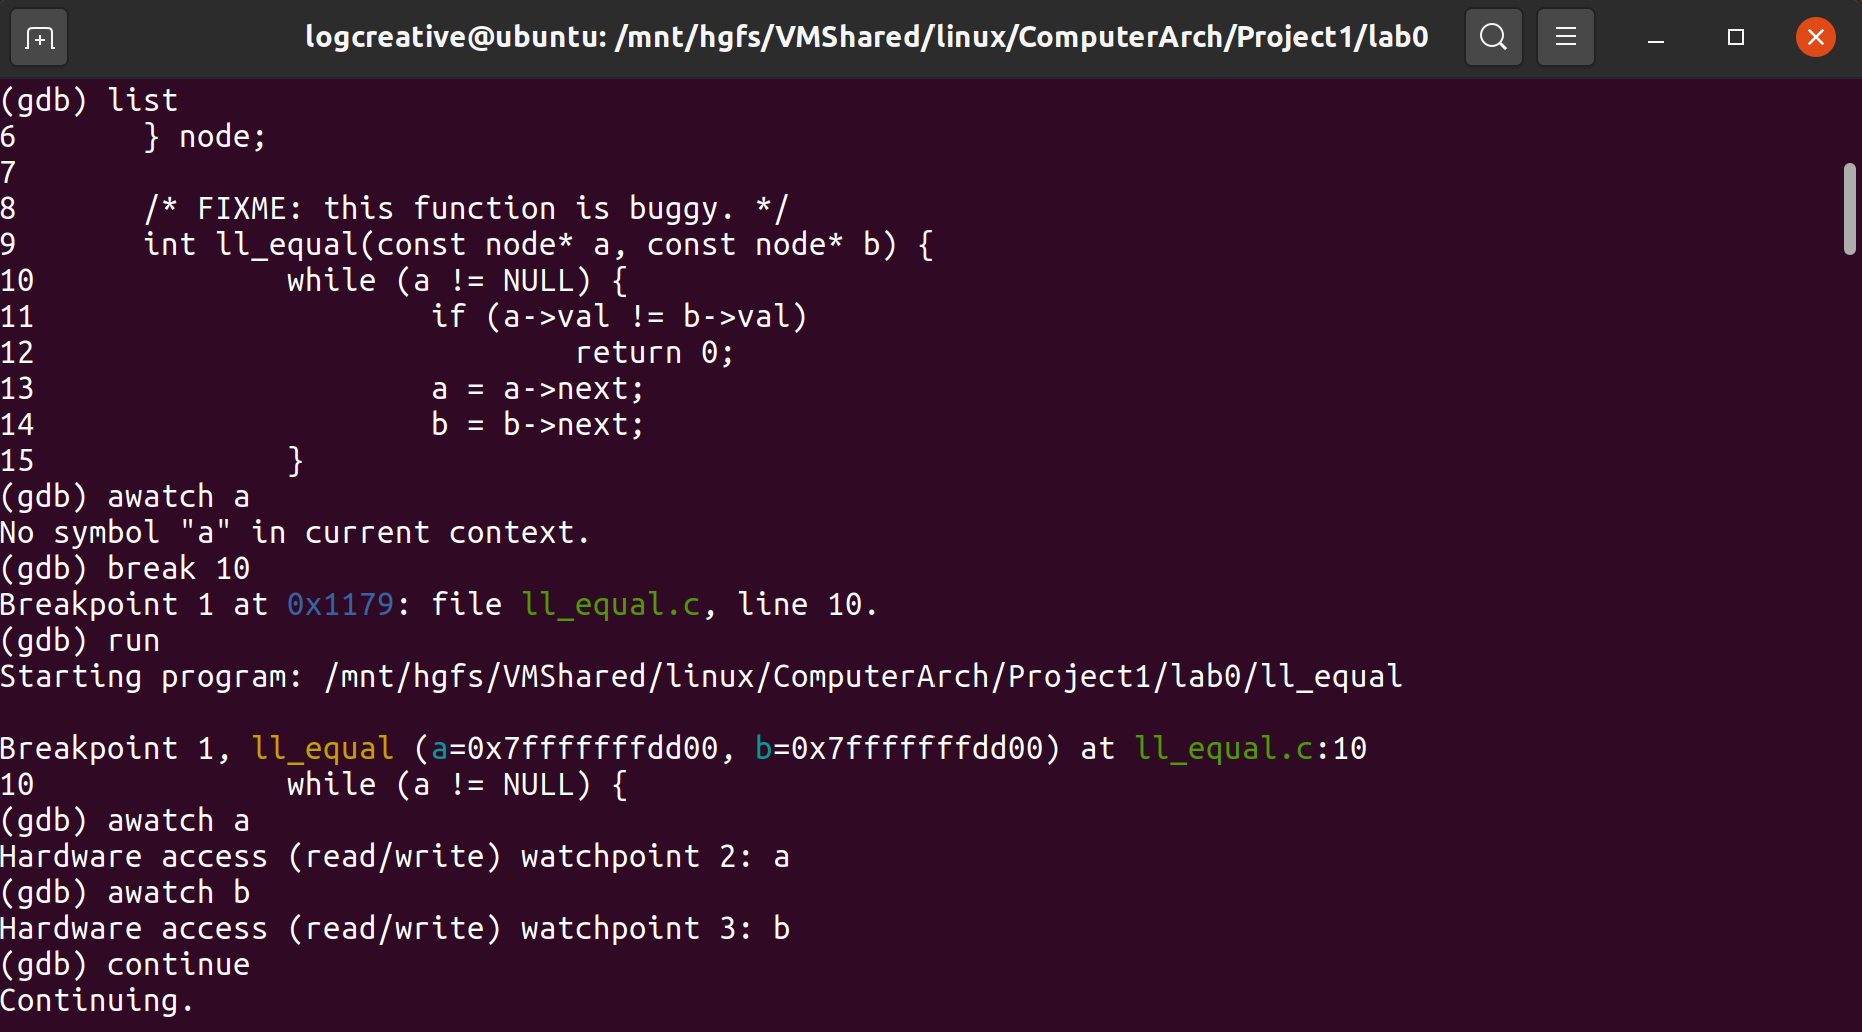
\includegraphics[width=0.9\textwidth]{debug.png}

    在进入第二轮测试时,出现错误。
    
    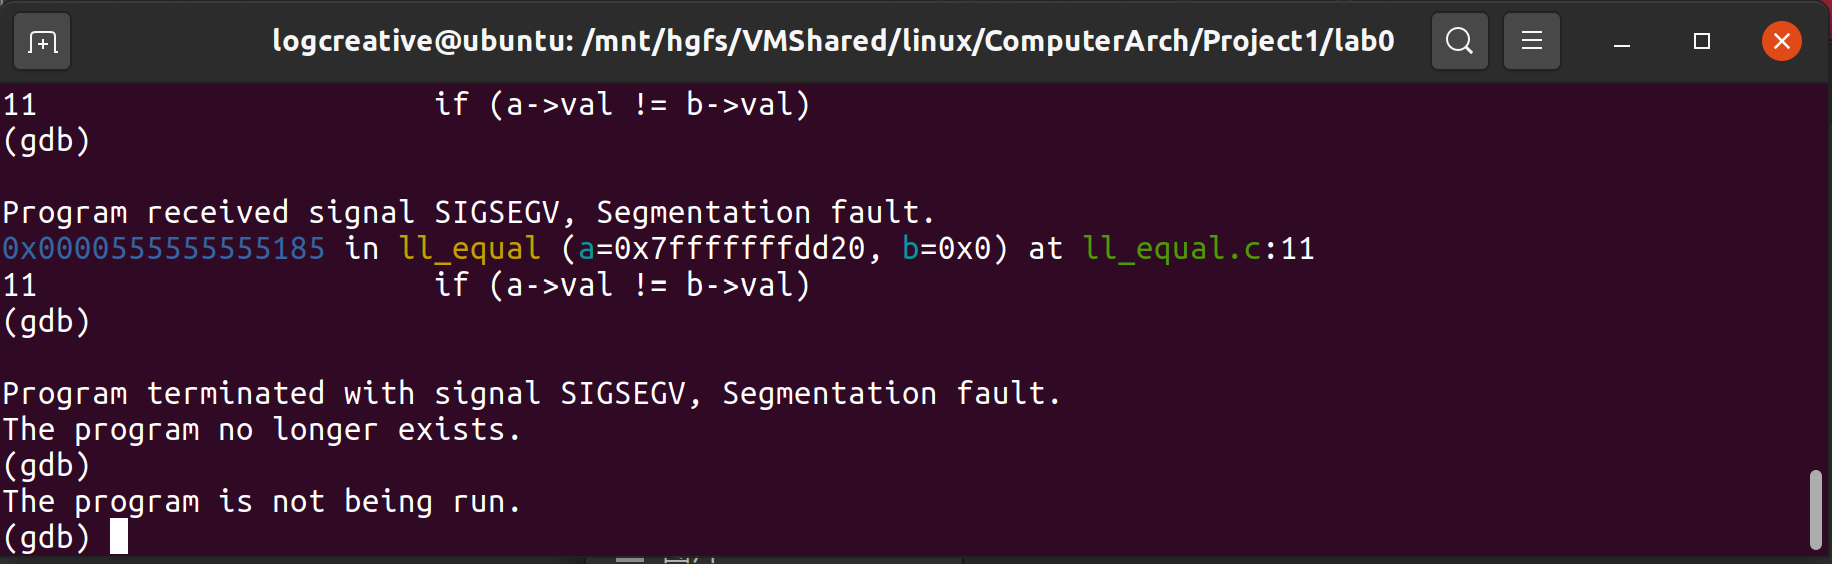
\includegraphics[width=0.9\textwidth]{fault.png}

    错误原因是 \texttt{b == NULL},空指针没有值。所以退出 \texttt{gdb},并在 Vim 修改
    \begin{code}{shell}
        vim ll_equal.c
    \end{code}

    更正后的函数如下:

    \begin{code}{c}
/* FIXME: this function is buggy. */
int ll_equal(const node* a, const node* b) {
	while (a != NULL && b != NULL) {
		if (a->val != b->val)
			return 0;
		a = a->next;
		b = b->next;
	}
	/* lists are equal if a and b are both null */
	return a == b;
}
    \end{code}

    之后就正常运行了:
    \begin{literal}
equal test 1 result = 1
equal test 2 result = 0
    \end{literal}

    \item[4] \texttt{make}
    运行几条指令:
    
    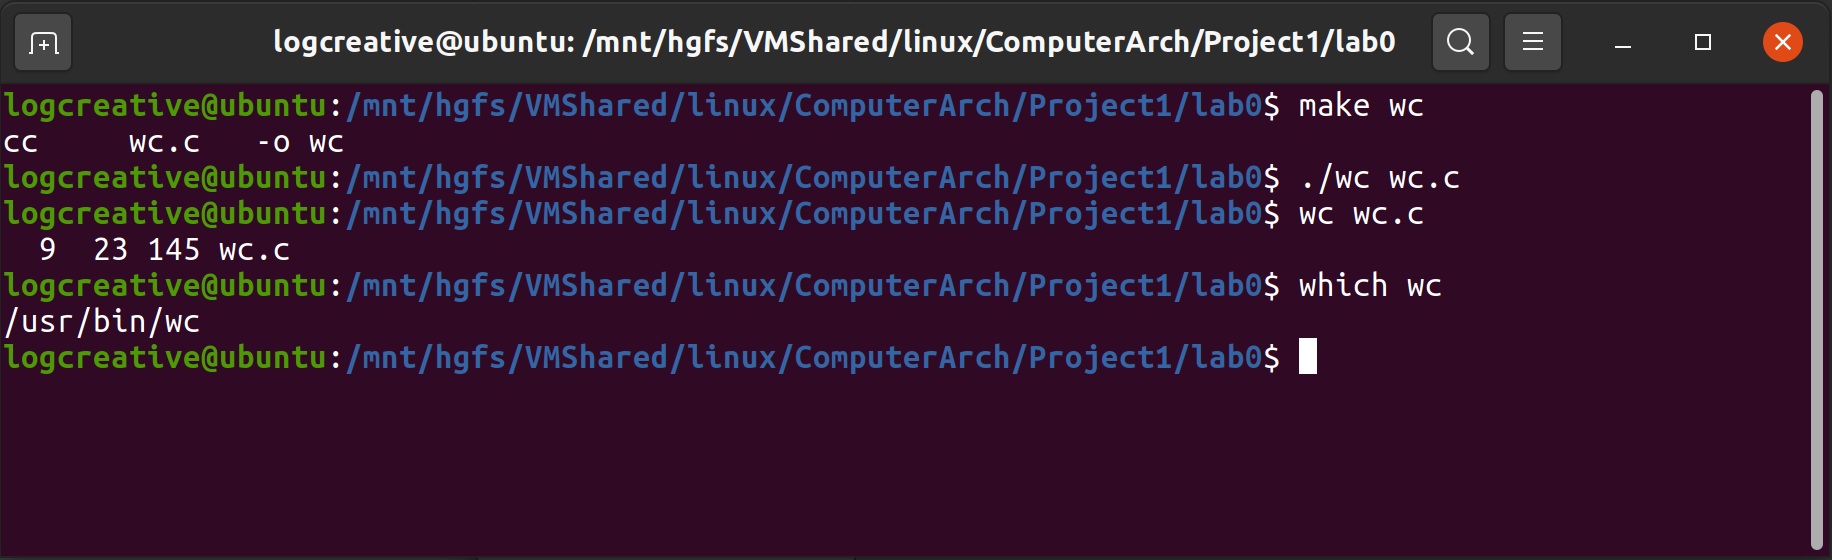
\includegraphics[width=0.9\textwidth]{make.png}

    \texttt{make} 指令编译 \fname{wc.c} 文件,使用 \texttt{./wc} 将会运行该文件,而只使用 \texttt{wc} 会调用系统指令,输入帮助指令
    \begin{code}{shell}
        wc --help
    \end{code}
    会得到帮助:
    \begin{quote}
        Print newline, word, and byte counts for each FILE, and a total line if more than one FILE is specified.
    \end{quote}
    会打印文件的行数、单词数、文件大小。

    仿照 Ubuntu 的 \texttt{wc} 命令,补充了 \fname{wc.c},当无文件名输入时,会计算用户的输入,运行结果如下:

    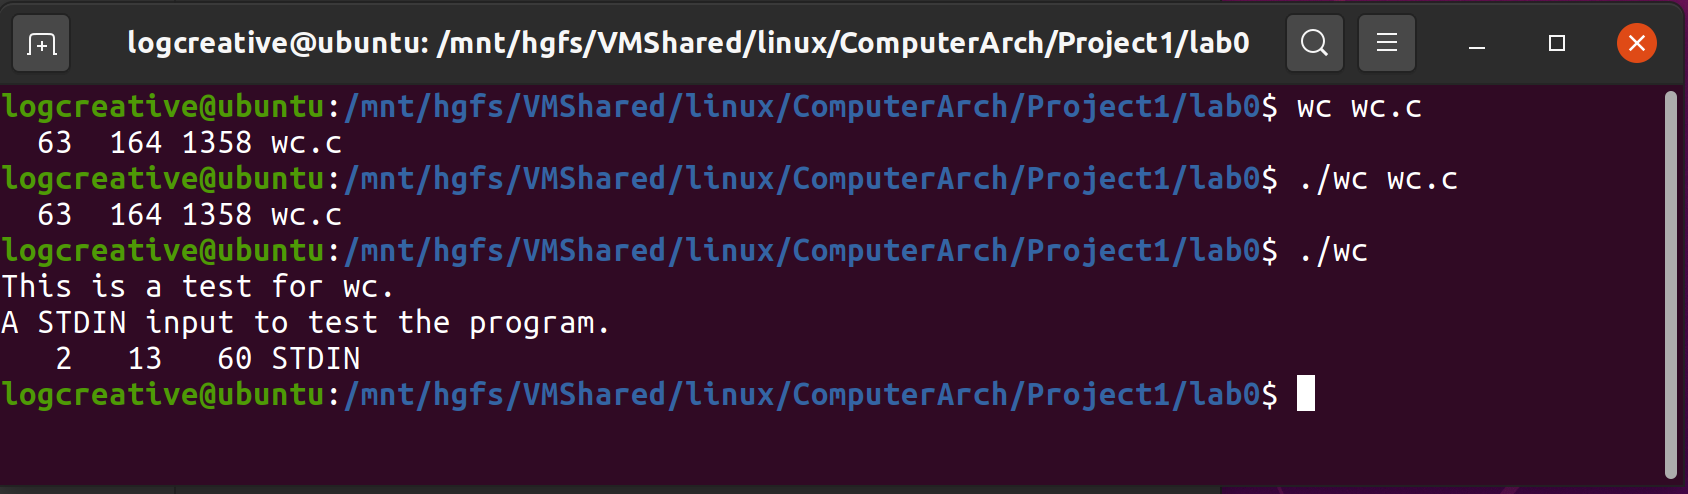
\includegraphics[width=0.9\textwidth]{wc.png}
    
    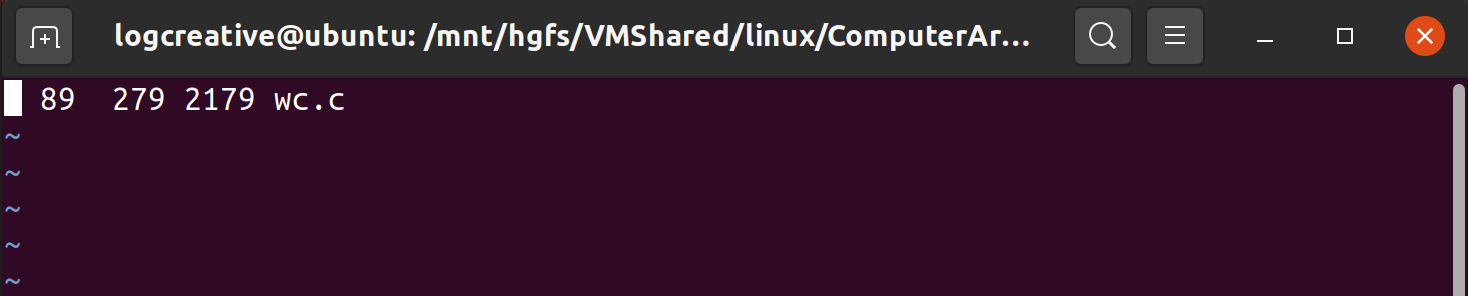
\includegraphics[width=0.9\textwidth]{wct.png}

    \fname{wc.c}
    \inputminted[breaklines,autogobble,linenos,numbersep=1mm,frame=lines,framesep=2mm,fontsize=\scriptsize,]{c}{../lab0/wc.c}

\end{problems}


\end{document}
